\documentclass{article}
\usepackage{todonotes}
\usepackage{biblatex}
\usepackage{listings}
\usepackage{color}
\usepackage{copyrightbox}
\usepackage{ccicons}
\definecolor{lightgray}{rgb}{.9,.9,.9}
\definecolor{darkgray}{rgb}{.4,.4,.4}
\definecolor{purple}{rgb}{0.65, 0.12, 0.82}
\lstdefinelanguage{JavaScript}{
  keywords={break, case, catch, continue, debugger, default, delete, do, else, false, finally, for, function, if, in, instanceof, new, null, return, switch, this, throw, true, try, typeof, var, void, while, with},
  morecomment=[l]{//},
  morecomment=[s]{/*}{*/},
  morestring=[b]',
  morestring=[b]",
  ndkeywords={class, export, boolean, throw, implements, import, this},
  keywordstyle=\color{blue}\bfseries,
  ndkeywordstyle=\color{darkgray}\bfseries,
  identifierstyle=\color{black},
  commentstyle=\color{purple}\ttfamily,
  stringstyle=\color{red}\ttfamily,
  sensitive=true
}

\lstset{
   language=JavaScript,
   backgroundcolor=\color{lightgray},
   extendedchars=true,
   basicstyle=\footnotesize\ttfamily,
   showstringspaces=false,
   showspaces=false,
   numbers=left,
   numberstyle=\footnotesize,
   numbersep=9pt,
   tabsize=2,
   breaklines=true,
   showtabs=false,
   captionpos=b
}
\bibliography{bibliography}

\begin{document}

\title{Multiple coordinated views of massive geo data using tree maps and choropleth maps}
\author{Robert Schäfer\\ Department of Computer Graphics, Hasso-Plattner-Institut}
\maketitle

\newcommand{\rufu}{\textsc{Rundfunk MITBESTIMMEN}}
\newcommand{\visan}{\textsc{visual analytics platform}}
\newcommand\hmm[1]{\ifnum\ifhmode\spacefactor\else2000\fi>1000 \uppercase{#1}\else#1\fi}
\newcommand{\cmv}{\hmm{c}oordinated multiple view}
\newcommand{\cmvs}{\hmm{c}oordinated multiple views}
\newcommand{\map}{\textsc{2D} map}
\newcommand{\maps}{\textsc{2D} maps}
\newcommand{\tmap}{\textsc{2.5D} tree map}
\newcommand{\tmaps}{\textsc{2.5D} tree maps}
\newcommand{\threedTmap}{\textsc{3D} tree map}
\newcommand{\threedTmaps}{\textsc{3D} tree maps}
\newcommand{\twodTmaps}{\textsc{2D} tree maps}
\newcommand{\dss}{\hmm{d}ecision support systems}
\newcommand{\riso}{\texttt{RISO}}
\newcommand{\attr}[1]{\texttt{\detokenize{#1}}}

\begin{abstract}
  Numerous visualization techniques exist for data-driven \dss{}.
  Two of which, namely tree maps and choropleth maps are especially useful when dealing with hierarchical and geographical data respectively.
  While a choropleth map is an sensible choice for geographical data, there is no obvious mapping of arbitrary hierarchical data.
  On the other hand, tree maps allow to visualize arbitrary, hierarchical and multidimensional data using nested rectangles.
  Although a tree map looks similar to a geographical map, the result may not be as intuitive and comprehensible.
  There is no predefined layouting for arbitrary data, let alone no well known layouting that everybody feels comfortable with.
  In this thesis, we propose and evaluate a coordinated multiple view to combine advantages of both visualizations.
  In one view, the user gets an easy access with a familiar geographical map, while in the other view the same data is displayed in a tree map.
  \todo[inline]{Should we mention the combination of multiple data sets here?}
\end{abstract}

\section{Introduction}
The human brain processes visual information better than it processes text.
As a result, the most tangible data analyses usually come with some sort of data visualization.
Data visualizations on a computer allow for user interactions and different levels of granularity according to the customer demands, which provides a great user experience.
There are a multitude of different techniques.
\cmvs{} take data visualizations to the next level by exploiting the respective advantages of the used visualizations as much as possible.
This combination may yield a greater value to the user, but it is unclear what kind visualization techniques work best together and for which kind of data.
How a user interact with \cmvs{} and how it differs from the use of single visualizations is another question worth to investigate.
In this thesis, we consider the question how a combination of a geographical visualization with a hierarchical visualization performs, for what kind of data this combination is suitable and what interaction patterns apply.

% Three moves
%\todo{What is the topic about?}
\todo[inline]{Establish the niche, why is there further research on your topic?}
\todo[inline]{Introduce the current research, what's the hypothesis, the research question?}

\subsection{Motivation}\label{sec:outline}

We create data visualizations of multi-dimensional, hierarchical and geographical data.
Namely, we develop \rufu{} which is an application for German citizen to publish which public broadcasts should benefit from their broadcasting fees.
The output of this application is a public user ranking and it can be used by broadcasting corporations to evaluate their program.
Data visualizations guide media researchers, journalists and the general audience to draw conclusions.
In this particular use case, the selection and interaction with the data may happen geographically, but the desired visualization could show e.g. changes over time or relationships within the data.

To explain this a little deeper:
Public broadcasting in Germany is organized federally, a German home belongs to the jurisdiction of a public broadcasting corporation.
But the produced content can be used all German citizen and it is even required to be free and available to everyone.
So this means that e.g. a media researcher might want to select all users from within a certain region, but is actually interested into relationships of broadcasts that are preferred by people from that area.

So the interaction and selection of data should happen in another view than the actual data visualization.
Since we deal with geographical data, we use geometry on a map for selection and interaction.
For the visualization, we use a different technique, e.g. a tree map if we deal with hierarchical data.

\todo[inline]{More scenarios here}

\subsection{Problem statement}

% \todo[inline]{Start off with the problem of tree map vs geo map}

\tmaps{} visualize hierarchical data on a two dimensional canvas and are particularly suitable if the proportions of the data should be emphasized.
When dealing with both multidimensional and geographical data, problems arise when other features than geographical features are used for the layouting of the \tmap{}.
As the order and placement of items depend on their specific values and hierarchy, items that should belong together according to their geographic circumstances may be scattered across the \tmap{}.
This obstructs the comprehensibility of map and makes it especially difficult to select geographical units of items.


\subsection{Research questions}

When dealing with multi-dimensional data, is it helpful to have multiple views for these dimensions?
What are best practices for the implementation of \cmvs{}?
Is it great user experience to have one view for interaction and another view for the data visualization to create insights?
Do people prefer one view for the interaction, e.g. the geographical dimension, or do they use all views for interaction and visualization alternately?

\subsubsection{Hypotheses}
Linkage and coupling of \cmvs{} can be enabled through visualizations, navigations and interaction techniques.
The exploration and analysis of multi-dimensional and geographical data can be supported with these \cmvs{}.
%Hypothese ist, dass durchs Visualisierungs-, Navigations- und Interaktionstechniken eine Kopplung von georäumlichen 2D-Kartendarstellungen und thematisch-orientierten 3D-Treemaps ermöglicht wird und dadurch die Exploration und Analyse von multidimensionalen georäumlichen Daten unterstützt werden kann.

\subsection{Objectives}

\todo[inline]{No section without text}


\paragraph{Basic \cmv{}}
The existing \visan{} is supplemented with a basic \cmv{} system.
Modules, interfaces and functionalities of the \cmv{} system are designed, coordinated and prototypically implemented.
In particular, a method for arranging multiple \cmv{} widgets in a \cmv{} layout and storing \cmv{} layouts is developed.

\paragraph{Interaction with the \cmv{}}
We develop coupling mechanisms and interaction mechanisms between \maps{} (for map-based representation) and \tmaps{} (for abstract information representation).
The functionality includes zoom per object or selection with a bounding box.
This creates a powerful selection mechanism, which can be used to select the data from the map-based representation in the \tmap{}.

\paragraph{Demonstration and evaluation}
\cmv{} layouts and suitable views are implemented and tested for the selected test data.
Based on the test data sets, the \cmv{} implementation is examined and evaluated for design criteria\cite{Baldonado2000}, general usability aspects\cite{Roberts2007} and usage for typical visual analytics tasks.
\todo[inline]{How elaborate is it to conduct a study for the usability of the \cmv{}? Who has done that before?}

% Our goal is to create meaningful data.
% This includes to encourage as many people as possible to publish their interests.
% It also involves to provide access to information about the preferred broadcasts.
% We suggest that users actively publish data and passively examine the summary of data of all users.
% Broadcasters on the other side receive the data and evaluate the program and actively change the program according to the interest of the audience.
% \todo[inline]{explain feedback loop}
% The mentioned data visualization need to be interactive to show the user the desired level of detail.

%\subsubsection{Use case specific goals}
%We propose the hypothesis that people behave differently when they decide consciously and when they decide with their remote control.
%The hypothesis goes even further, explicit interests may fit to the programme mandate of public broadcasting in contrast to TV and radio ratings which are based on usage data.

%As the data is usage independent we want to gain knowledge about the entire population including those who don't use broadcasting at all.
%In this manner we want to tackle the mentioned overfitting problem.

\subsection{Methodological approach}

A literature research is used to gather knowledge about the state of the art with respect to \cmvs{}.
Existing concepts and implementations available on the internet are examined and reused if possible.
Interviews of people from the target group are conducted and the define the requirements for the application.
A minimal viable product is developed to further validate the user requirements.
Also, common user behaviour is observed during user tests.
The prototype is continuously developed to allow for further experimentation.

\paragraph{Scenarios}
While implementing more features, we have two scenarios with different kind of data and different user requirements:
\begin{itemize}
  \item
    In our work on the project \rufu{} we design and prototype visualizations for media researchers.
    We fully control the database and the database schema as well as on the user facing application on top of it.
    User requirements are tied to journalists, media researchers, broadcasting corporations.
    The data has geographical, hierarchical, temporal and correlated characteristics.
  \item
    The \visan{} for administrative data is used as a more general purpose application.
    There is no single database schema but combatibility with many sources or services.
    User requirements are potentially unknown and part of the resarch.
    The usage focuses especially on geographical and hierarchical data.
\end{itemize}

For the scope of this master thesis we therefore compare implemented visualization and views.
How do both approaches differ in development speed, value for the customer?
What considerations need to be done regarding the database schema?

\todo[inline]{What is the area(s) of research, in which this thesis can be placed into?}
\section{Structure of the work}

In section~\ref{sec:research} we will give an overview on \cmvs{} and focus on visual analytics as well as massive, geographical data.
Existing concepts and implementations of \cmvs{} are examined and summarized in an overview.

\newpage

\section{State of the art}\label{sec:research}
Data visualizations are a key part in data-driven \dss{}\cite{Nada2007}\cite{Poleto2015}.
\textcite{Few2013} mentions sense-making (also called data analysis) and communication as some of the most important purposes of data visualization.
Statistical information is abstract and in data visualization ``we must find a way to give form to that which has none.''\cite{Few2013}

Visualizations are an obvious choice for managers who demand a quick overview on performance data.
In fact \textcite{Kusinitz2014} explains that the human brain processes visual information 60,000 times faster than text and visual content makes up even 93\% of all human communication.
Data visualizations are essential here, as managers often do not have the resources to do an in depth analysis with the numbers only.
We can expect to see these technologies more in more in business applications.
\textcite{McAfee2012} from the MIT Center of Digital Business showed that organizations driven most by data-based decision making had 4\% higher productivity rates and 6\% higher profits.
However, little research has been done regarding the performance of \cmvs{} in the field of decision making.
There might be a great potential.
Back in 1997 \textcite{Mayer1997} conducted eight studies to compare the effect of using multimedia on university students.
The studies showed that when using combined visual and verbal explanations the generation of creative problem solutions increased by an average of more than 50\%.

So the application of combined data visualization techniques in decision making seems to be a promising strategy.
Nevertheless is is unclear, which visualization techniques are the most suitable to be used in combination.
If we know what kind of data we are dealing with, what are the best suited visualization techniques?
Let's say we have multidimensional data, is there an order in how people access these multiple dimensions?
How do these visualizations perform and what are best practices to be considered for their implementation?

\subsection{Data related challenges}
\todo[inline]{Add independent section and explain tasks like data cleansing or data reliability regarding different sources here}



\subsection{Visualization of hierarchical data}
Due to the hierarchical nature of the of our use cases, we focus on the visualization of hierarchical and geographical data
The visualization of hierarchical data has a long tradition.
The traditional representation of a tree is a rooted, directed graph with the root node at the top.
An everyday use case is a directory tree example of a file system, e.g. in file browsers or command line utilities like \texttt{tree} in UNIX.
As \textcite{Shneiderman1992} mentions, this visualization becomes increasingly large when displaying more than one node and soon exceeds the entire screen size.
\textcite{Johnson1991} proposes the tree map visualization technique, in which each node is a rectangle whose area is proportional to some attribute, thus making 100\% use of the available screen size.
As we can see in figure~\ref{fig:research:treemap} large boxes are labeled with generic tems like ``cars'' and ``medicaments'' and include smaller boxes with more specific meanings.
We apply the same rules to ordinary maps.
The world can be divided into continents, which can be divided into countries, which can be divided into provinces and so on.
The difference is that there is no predefined algorithm for layouting, which brings up one of the major disadvantages of tree maps:
As the order of placement depends on the respective features of the nodes, small changes in the input data can lead to a large change in the layout of the resulting tree map.
%\todo{What are tree maps?}

\begin{figure}[h]
\centering
  \copyrightbox[b]{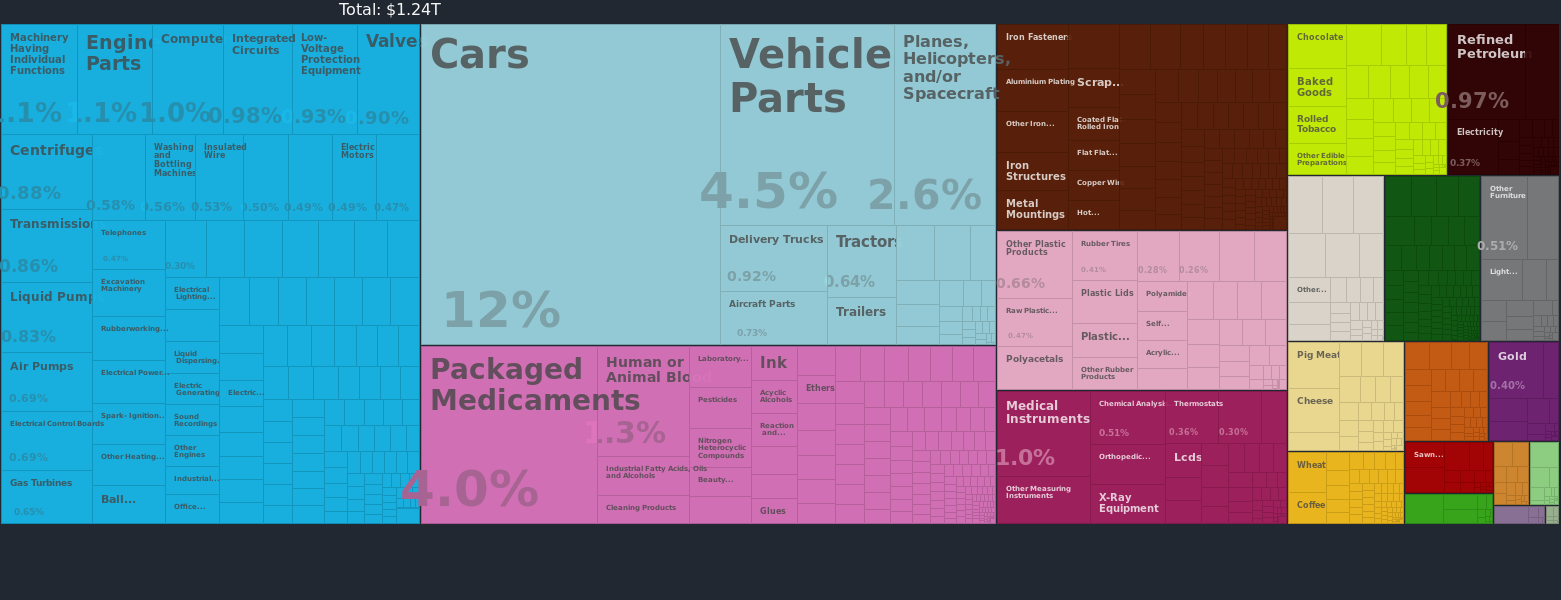
\includegraphics[width=\textwidth]{images/treemap_example}}{ \hfill \ccAttribution \ccShareAlike \hspace{1mm} Observatory of Economic Complexity\cite{Macro2017}}
\caption{German exports visualized as a tree map}
\label{fig:research:treemap}
\end{figure}

\subsubsection{\threedTmaps{} and \tmaps}

In 2004, \textcite{Bladh2004} transfer the concept of tree maps from two dimensional into three dimensional space.
The introduce StepTree, which is a three dimensional tree map to display a directory layout.
It ``differs from Treemap in that it employs three dimensions by stacking each subdirectory on top of its parent directory.''\cite{Bladh2004}
3D tree maps are superior to 2D tree maps for tasks with a pronounced topological challenge.
User perform significantly better in interpreting the hierarchical structure.
However, 3D visualizations also introduce some disadvantages as superimposition of objects and a complex view point navigation.

\textcite{Limberger2016} introduce the concept of a \tmap{} which is a constrained \threedTmap{}.
A \tmap{} has all items attached to the ground.
For the rest of this thesis, we will refer to this type of tree map.
We can see an example of a \tmap{} in figure~\ref{fig:research:ua_treemap}

\begin{figure}[h]
\centering
  \copyrightbox[b]{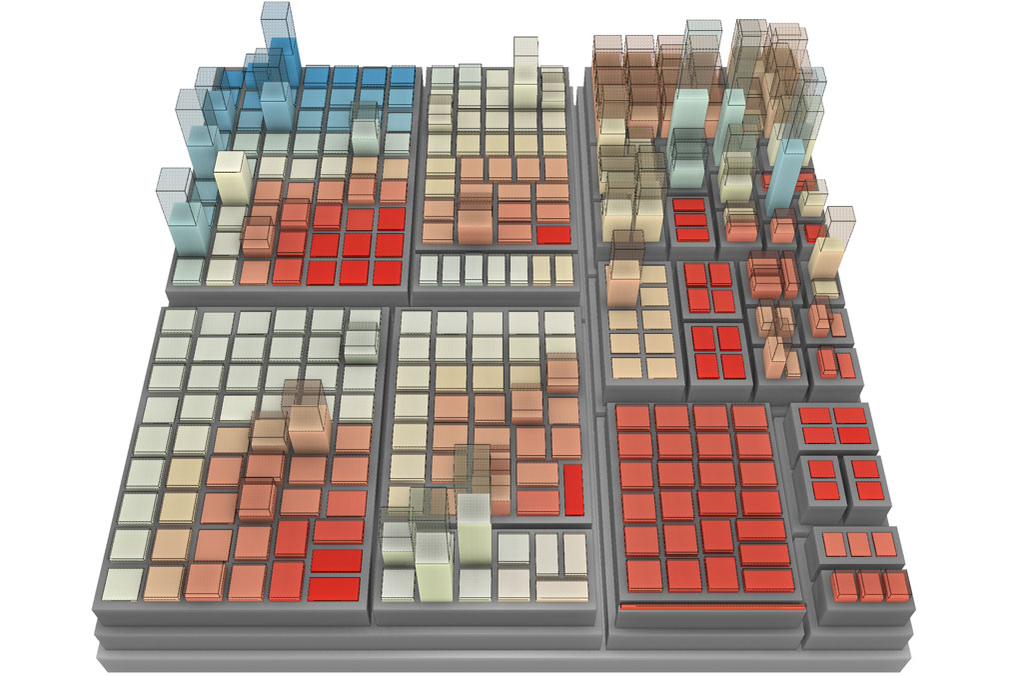
\includegraphics[width=\textwidth]{images/2_5D_treemap_example}}{ \hfill \textcopyright \hspace{1mm} Hasso-Plattner-Institut\cite{Doellner2017}}
  \caption{Example of a \tmap{}}
\label{fig:research:ua_treemap}
\end{figure}


\subsection{Choropleth map}
A choropleth map is a thematic map in which areas are shaded or patterned in proportion to the measurement of the statistical variable being displayed on the map.
A popular use case is the display of population density or per-capita income.
We can see an example of a choropleth map in figure~\ref{fig:research:choropleth}.
Choropleth maps are extremely popular and so the audience is likely to understand them.
They are very helpful when data is attached to enumeration unites like counties, provinces and countries.

\begin{figure}[h]
\centering
  \copyrightbox[b]{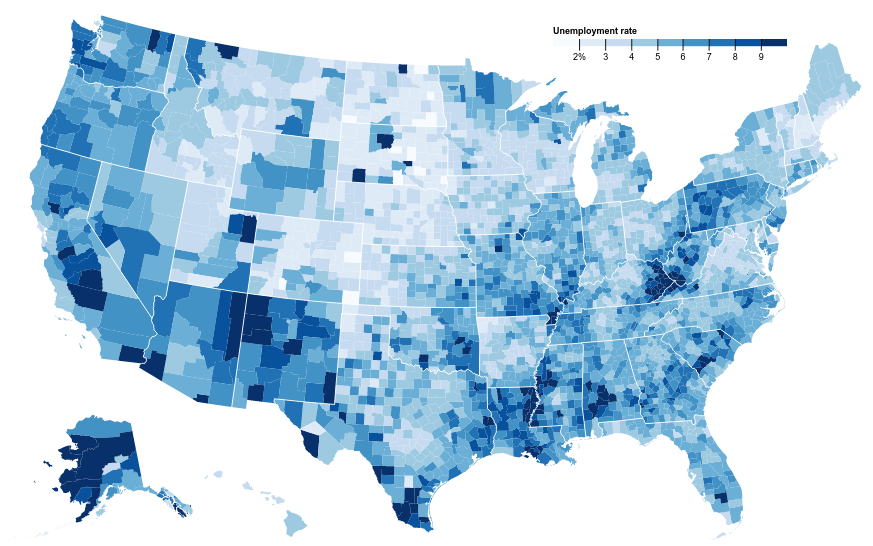
\includegraphics[width=\textwidth]{images/choropleth_example}}{ \hfill GPLv3 Mike Bostock\cite{Bostock2017:2}}
  \caption{Unemployment rate in the USA}
\label{fig:research:choropleth}
\end{figure}

\todo[inline]{How do tree maps relate to geographical data?}

\subsection{Coordinated multiple views}
According to \textcite{Roberts2007} \cmvs{} is just ``a specific exploratory visualization technique that enables users to explore their data''.
\cmvs{} are characterized by the fact, that they show multiple views side-by-side.
Most multiple coordinated views also provide some kind of brushing technique.
``The technique of brushing is the principle approach, where elements are selected (and highlighted) in one display, concurrently the same information in any other linked display is also highlighted.''\cite{Roberts2007}
%\todo{What are CMVs?}
We can see an example in figure~\ref{fig:research:cmv}.
It displays an on-time performance of airlines, visualized with the ``Crossfilter'' javascript library.
The user can set the borders of an interval with the mouse in each of the views.
The visualization takes the most recent 80 flights from the database that match all given filters.
All visualizations are then updated in real time.
As we can see in the example in figure~\ref{fig:research:cmv} there seems to be a correlation of a long delay with a later time of the day.

\begin{figure}[h]
\centering
  \copyrightbox[b]{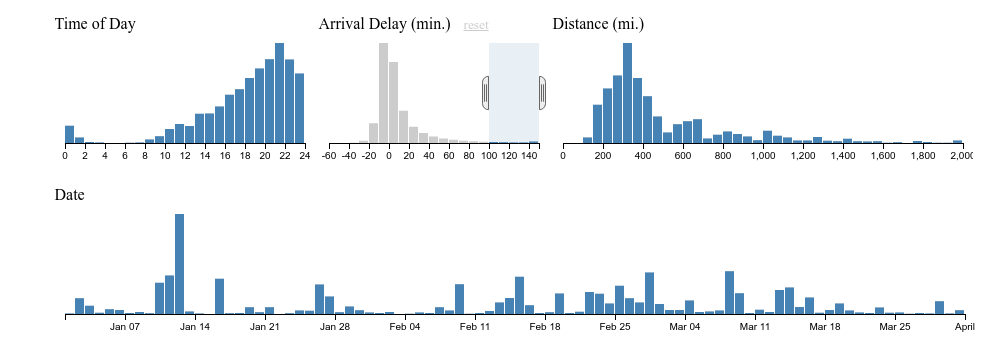
\includegraphics[width=\textwidth]{images/cmv_example}}{\hfill Crossfilter\cite{Bostock2017}}
\caption{Airline on-time performance: Correlation of time of day with arrival delay. Most recent flight with a delay of more than 100 minutes selected.}
\label{fig:research:cmv}
\end{figure}

\section{Concept}

Since we deal with real world problems, we aim to evaluate the developed tools on real users and existing data.

\subsection{Data sets}
For our uses cases, we have two different data sets:
One data set consists of a user ranking of public broadcasting in Germany, i.e. entities, mostly TV and radio broadcasts, are liked or disliked by people.
This data is public data and can be used by media researchers of broadcasting corporations but also targets media journalists and the general audience.
The other set, called \riso{}, consists of statistical data from various German administrations and is used by the authorities for urban planning and policy strategies.

Both data sets share some characteristics.
The administrative data connects certain features with certain regions of Germany.
As Germany is a federal state, larger regions consist of many other smaller regions.

The second one consists of user data that was collected through a web application called \rufu{}.

\subsubsection{RISO}

The \riso{} data base is used in by local authorities to get insights about governmental KPIs to assist local and regional decision making.
It is a relational database and a part of the data base schema is shown as an ER diagram in figure~\ref{fig:data:riso}.
\begin{figure}[h]
\centering
  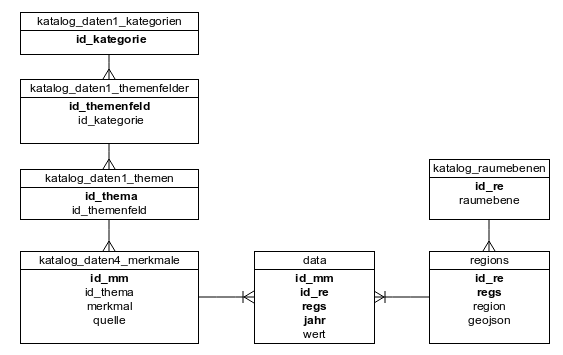
\includegraphics[width=\textwidth]{images/riso}
  \caption{Part of the \riso{} database schema. Primary keys are set in bold.}
  \label{fig:data:riso}
\end{figure}

The largest table is called \attr{data} with approximately 10,466,600 records, which holds all values along with the survey date.
\paragraph{Features}
This data is connected to a feature table through a foreign key called \attr{id_mm}.
In the feature table we can find the description for every referenced feature, e.g. population density, working population in agriculture, education spending.
The \riso{} system groups all features in a 4-level hierarchy:
\begin{enumerate}
  \item
    \attr{katalog_daten_1_kategorien}
  \item
    \attr{katalog_daten_2_themenfelder}
  \item
    \attr{katalog_daten_3_themen}
  \item
    \attr{katalog_daten_4_merkmale}
\end{enumerate}
The actual features table is the last one in the list.
At the lowest level within the hierarchy, this is the largest table with 1234 records.


\paragraph{Regions}
On the other side, the geographical data is stored in the \attr{regions} table.
The geometry data for each region is stored in the \attr{geojson} column and as the name suggests, the data type is a \attr{geojson}.
The foreign keys that connect the tables \attr{data} and \attr{regions} are called \attr{id_re} and \attr{regs}.
Unlike the feature table, the regions are grouped through the \attr{id_re} that indicates the hierarchy level.
So the values of the \attr{id_re} column denominate the level of the hierarchy.
E.g. a region with a \attr{id_re} of $1$ is a federal state of Germany, a region with id $13$ is a constituency.
A textual description for the hierarchy level can be found in the \attr{katalog_raumebenen} table in column \attr{raumebene}.
Both column \attr{id_re} and \attr{regs} belong to the primary key of the regions table, so there will never be two regions on the same hierarchy level with the same \attr{regs} id.

\paragraph{Characteristics}
As we can see, the schema of the \riso{} database follows a rather denormalized approach.
The schema does not make a lot of assumptions regarding the input data.
It allows to add data of arbitrary size, features and completeness as long as there is some kind of numerical data associated with some kind of geographical unit.
This approach is suitable for a data base that incorporates data from different sources, as it is the case with the \riso{} data base.


\subsubsection{\rufu{}}
Unlike the \riso{} database, the data base of \rufu{} is used as persistency layer.
For that reason the data base schema follows the requirements of a productive web application.

As outline in section~\ref{sec:outline} \rufu{} is an evaluation platform for public broadcasting in Germany.
First, users vote on broadcasts, i.e. they decide if they want to support broadcast or if they do not want to support.
As a next step, user can then make a priorisation by distributing a virtual, monthly budget among the chosen broadcasts.

Figure~\ref{fig:data:rundfunk} shows the data base schema of the application.
A \attr{user} is connected to \attr{broadcast} through a \attr{selection}.
If the \attr{user} supports some a broadcast, the \attr{response} on the given \attr{selection} will be `positive'.
If the \attr{user} does not wish to support a \attr{broadcast}, the \attr{response} will be `neutral'.
The \attr{user} can allocate virtual money to supported broadcasts.
The money will be stored in the column \attr{amount} of the \attr{selection}.
The sum of all amounts for one user will never exceed the virtual budget of 17.50€.

\begin{figure}[h]
\centering
  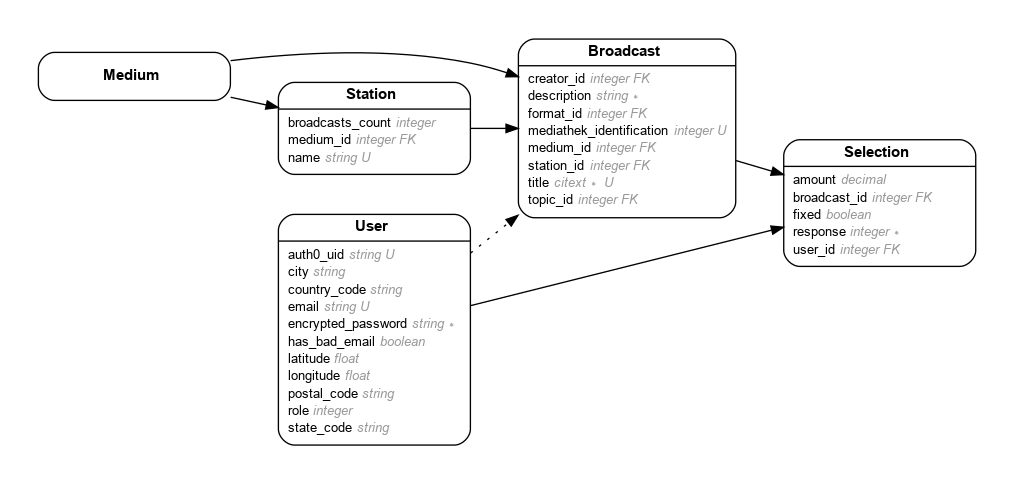
\includegraphics[width=\textwidth]{images/er}
  \caption{Database schema of the \rufu{} app}
  \label{fig:data:rundfunk}
\end{figure}

\paragraph{Features}
We have both numerical as well as nominal features.
A numerical feature could be the number of supporters from an area in Germany.
A nominal feature could be a list of the most supported broadcasts from an area in Germany.
Numerical and nominal features can be combined, so we could request for every region, a distribution of the desired expenditure for radio, TV, online and other broadcasts.

\paragraph{Regions}
\rufu{} stores the geometry for each region in \attr{geojson} files.
This file holds a \attr{FeatureCollection}.
Every \attr{Feature} is a region, the identifier is stored as a property.
We merge the geometry data with features for every request.
To be precise: We get all the user data, group it by the identifier \attr{state_code} and merge it with the geometry in the \attr{geojson}.

\paragraph{Characteristics}
The data base schema is a result of the specific requirements of a persistency layer.
Changes in the source code may require a migration of the data base schema.

However, we can ask a lot of questions already with common data base queries or standard data analysis tools:
\begin{enumerate}
  \item
    How does the actual support of a broadcast compare to the average support of a broadcast?
  \item
    What are the most popular broadcasts in Berlin?
  \item
    What is the desired ratio of genres of supported broadcasts? How important is education compared to sport?
  \item
    How does the support of a broadcast change over time?
  \item
    According to the user ranking, which broadcasts are similar to each other?
\end{enumerate}


\subsection{Implementation}

An example of aggregated user data merged with geometry data can be seen in listing~\ref{lst:geojson:example}.
\lstinputlisting[language=JavaScript, label={lst:geojson:example}, caption={Geojson example}]{listings/example.geojson}

We can use this data as input for our common \visan{}, e.g. figure~\ref{fig:implementation:user_distribution} shows the user distribution of \rufu{}.

\begin{figure}[h]
\centering
  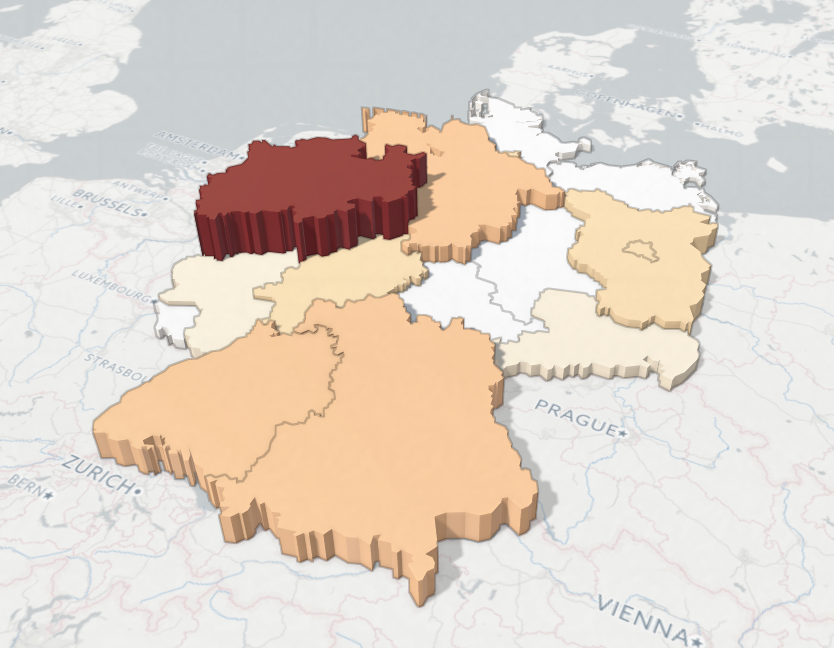
\includegraphics[width=\textwidth]{images/ua_example.png}
  \caption{User distribution of \rufu{} across German federal states}
\label{fig:implementation:user_distribution}
\end{figure}


\clearpage
\section{Implementation}

This section describes the implementation details for the described concepts.
We start with a list of to be implemented features.
Next, we describe the architecture of the software and why we chose this architecture.
What requirements and considerations lead to this particular architecture.

\subsection{Interaction techniques}
\textcite{Yi2007} lists seven categories of interation in information visualization:
\begin{enumerate}
  \item
    \textbf{Select} mark something as interesting
  \item
    \textbf{Explore} show me something else
  \item
    \textbf{Reconfigure} show me a different arrangement
  \item
    \textbf{Encode} show me a different representation
  \item
    \textbf{Abstract/Elaborate} show me more or less detail
  \item
    \textbf{Filter} show me something conditionally
  \item
    \textbf{Connect} show me related items
\end{enumerate}

\subsubsection{Existing interactions}
The possible inteactions in our current \visan{} can be categorized \emph{select}, \emph{explore}, \emph{reconfigure}, \emph{encode} and \emph{filter}.
As seen in figure~\ref{fig:implementation:interaction:existing} the user can \emph{select} one item in the view by clicking on it.
The user can reveal a tooltip showing the item properties by hovering with the mouse on the item, which is another \emph{selection}.
The user can \emph{explore} the map in the usual manner:
If the user drags with the mouse on the map, a panning operation is performed with the viewpoint focused on Germany, i.e. the camere moves around like a turntable.
The zoom factor can be changed by scrolling on the canvas of the map.
\emph{Encode} and \emph{reconfigure} techniques are performed through the menu on the left side:
Under the ``features'' tab, the user can \emph{reconfigure} different data sets and the displayed diagram, e.g. a tree map visualization based on the geometry shape, cubes or voronoi regions.
The tab ``Dimensions'' allows the user to \emph{encode} properties of a data set to visual attributes, e.g. the height, color and texture of an item.
The tab ``Filter'' can be used to reduce the displayed data set along a range of continuous values.
Figure~\ref{fig:implementation:interation:existing:filter} shows the range of visible values in the left menu.
When the user drags the slider, the items in the map on the right side are updated interactively.

\begin{figure}[h]
\centering
  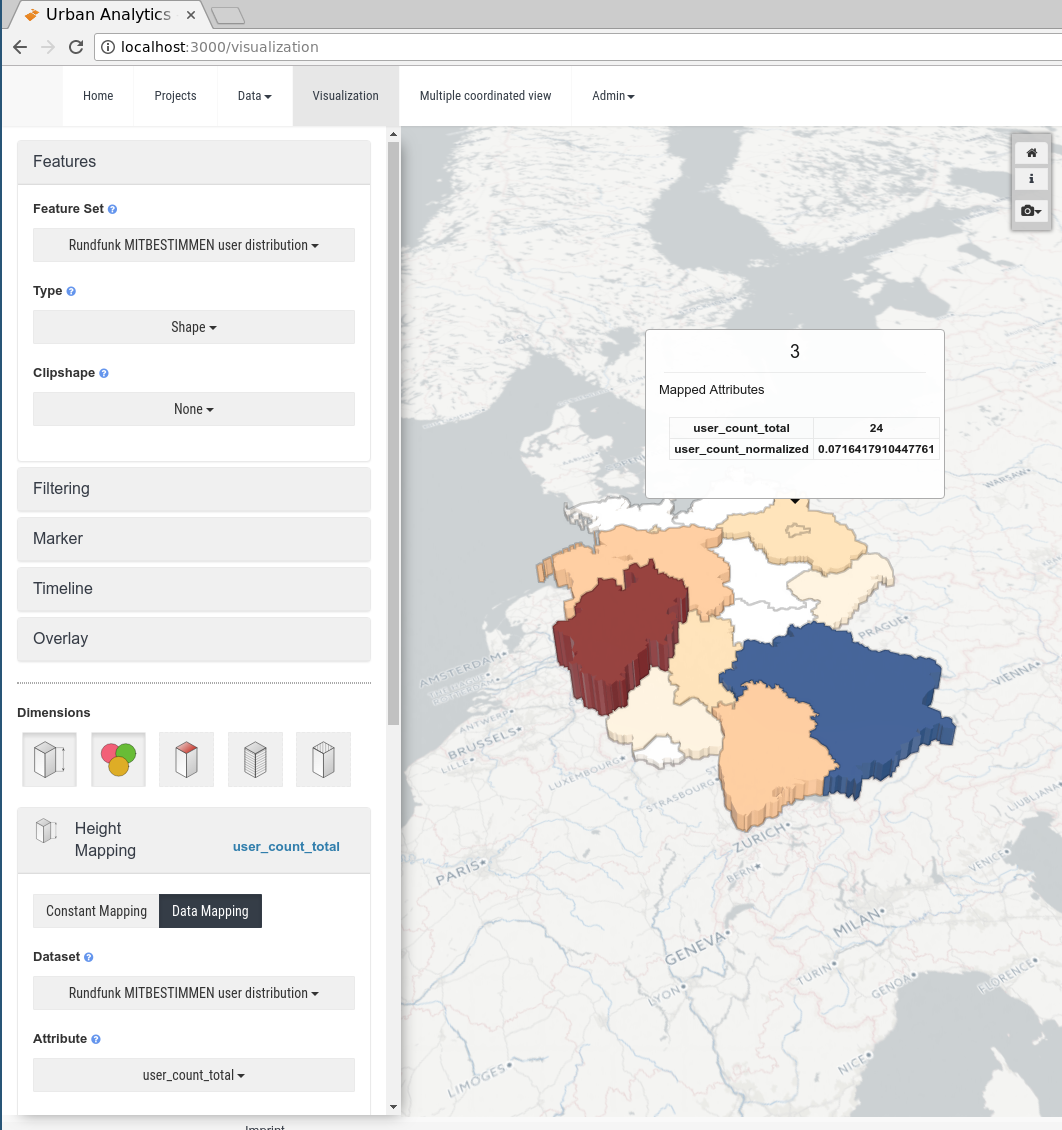
\includegraphics[width=\textwidth]{images/implementation-interaction-existing.png}
  \caption{
    Items can be highlighted with a click, Bavaria is currently highlighted.
    A mouse over reveals a tooltip showing item properties.
    The menu on the left side allows to change the data set and the specific base visualization.}
  \label{fig:implementation:interaction:existing}
\end{figure}

\begin{figure}[h]
\centering
  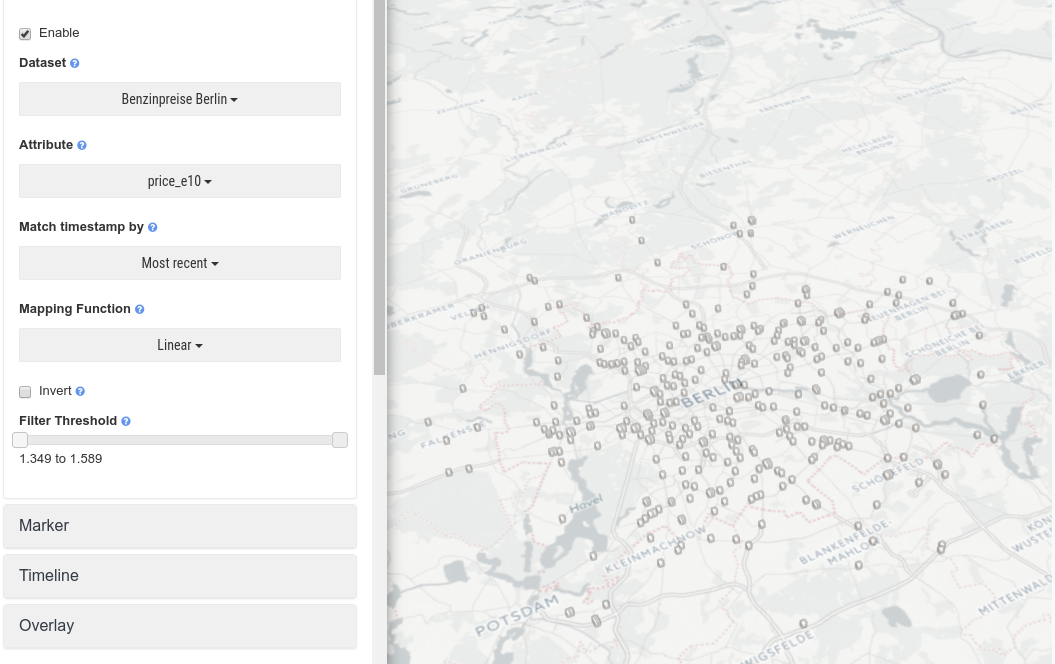
\includegraphics[width=\textwidth]{images/implementation-interaction-existing-filter.png}
  \caption{ Only gas stations with a price for E10 within 1.349 Euro and 1.589 Euro are displaeyd in the map}
  \label{fig:implementation:interaction:existing:filter}
\end{figure}

\subsubsection{Implemented interactions}

In the course of this thesis we want to implement the following interactions:
\begin{itemize}
  \item
    \emph{Select}: The user clicks on a building or region in a geographical map and all affected properties in the \tmap{} will be highlighted.
  \item
    \emph{Explore}: The user clicks on a block in the \tmap{} and the viewpoint in the geographical map will be centered on relevant area.
  \item
    \emph{Abstract/Elaborate}: The user selects a different granularity in the geographical map (e.g. postal code regions instead of federal states) and the change is reflected in the \tmap{}.
  \item
    \emph{Filter}: The user double-clicks on a region in a geographical map and the \tmap{} will be based on data of only that region.
\end{itemize}

\paragraph{Component pattern}
State-of-the-art javascript frameworks like ReactJS and EmberJS follow the component pattern for the architecture of a single page web application.
The component pattern imposes a hierarchical structure on a website.
Each component is responsible for a task and may contain other components.
The components are joined at the root node of the page.

This pattern is very applicable to \cmvs{}.
The different views of \cmvs{} share state, i.e. the feature, that is currently highlighted or the applied filter on the data.
So the views are components and their closest common ancestor is the \cmv{} itself, controlling state and passing user interaction down to it's children.

\paragraph{Actions up - Data down}

Version 2.0 of Ember introduced a common phrase how to use this pattern effectively: ``Data down, actions up''\cite{Emberigniter2017}
In the domain of \cmvs{} actions would mean user interactions, e.g. a click on a feature.
The action will notify the controlling \cmv{} component.
Actions may change data, and the changes will be passed to to all dependen views.
These views are then rerendered.

Examples for the kind of data that might trigger a rerendering of a view:
\begin{itemize}
  \item
    The selected feature or a list of selected features
  \item
    A list of thresholds for certain features as a filter
\end{itemize}

\paragraph{Web components}

Web components is a recent standard of the W3C\cite{W3C2017} to bring component-based software engineering to the world wide web.
They look perfectly suited to be used in \cmvs{}.
However the attributes of web components are string based.
If arbitrary javascript objects need to be passed into the web component it is suggested to use one of the common javascript frameworks that allow for data binding.



\clearpage
\printbibliography
\end{document}



%\subsubsection{Use case specific problems}
%There is striking discrepancy of intentions between available metrics and the programme mandate of public broadcasting.
%TV ratings are produced by a group of 5000 representative homes equipped with a special TV box, while Radio ratings are carried out by phone surveys over the course of a year.
%Although created differently they share the same intention, i.e.\ to sell advertisements.
%
%We suspect that public broadcasting suffers from an overfitting problem:
%Since broadcasters have usage data only, they focus too much on people who still listen to the radio and watch TV.
%Young people especially show a decreasing interest in conventional mass media which has been shown in surveys.
%Public broadcasting fails in that respect that everybody has to pay and thus has a right to get access to information.

%In many cases, insights based on visualization techniques like \cmvs{} are used by experts for strategic decision-making.
%Thus, many advanced data visualizations techniques are made exclusively for professionals.
%
%On the other hand, data visualizations widely popular:
%Data journalism is one of the emerging fields in journalism.
%Facts and figures are the strongest evidence for opinionated journalistic reports.
%Not even a football match can do without a number based analysis.
%
%We believe that advanced data visualization techniques can be adopted and used in both an informative and strategic way by professionals as well as lay people.



% We use data visualizations in the context of the expenditure of public broadcasting fees in Germany.
% Since the year 2013 these fees are compulsory for every home in Germany and as a consequence, broadcasting receives €8,000,000,000 annually.
% Yet it is subject to little or no public feedback, ranking, or even debate on what constitutes value or quality.
% There is neither transparency on how the fees are spent nor a public feedback on how the fees should be spent.
% 
% We see a great potential, a win-win situation to be precise, because both payers of the broadcasting fees and broadcasters themselves can benefit from each other.
% As of 2013 there is no legal opt-out anymore and people have a strong interest to say how their fees should be spent.
% Broadcasters on the other hand can evaluate their program based on the interests delivered by the users.
% This reciprocal relationship would create a public feedback for payers and a better program for broadcasters.
% 
% This problem is perfectly suitable to be tackled with data visualizations.
% \todo[inline]{Explain why data visualization are good for communication}

%Our use case is creating a tool to publicly evaluate public broadcasting in Germany.

%Public broadcasting has a long history in all of Europe.
%Especially after the experiences of the Third Reich, freedom of the press and freedom of broadcasting in particular was defined in the German constitution, the basic law.
%Article 5 not only ensures the press to be free of censorship.
%It is interpreted in such a way that it guarantees broadcasting to exist and be politically and economically independent.
%It is remarkably in many ways:
%First, mass media are recognised to be a basic prerequisite for formation of opinion of the general public.
%Second, the state fosters free access to information, ie. Open Knowledge.

%Despite this highly positive ideal, reality looks somewhat different.
%Public broadcasting in Germany receives €8,000,000,000 (eight billion euros) annually, yet it is subject to little or no public feedback, ranking, or even debate on what constitutes value or quality.
%Since 2013, there is no legal opt-out for German citizen anymore.
%Every home in Germany has to pay for broadcasting whether or not the people actually use it.
%This has created numerous constitutional complaints and approximately 2 million homes in Germany refuse to pay, even it is virtually illegal to do so.

